% Chapter 7

\chapter{Findings and Discussion} % Main chapter title

\label{Chapter7} % For referencing the chapter elsewhere, use \ref{Chapter1} 

\lhead{Chapter 7. \emph{Findings and Discussion}} % This is for the header on each page - perhaps a shortened title

%----------------------------------------------------------------------------------------
\section{Summary of contribution}
The document presents an approach of implementing a dynamic energy map
with a focus on visualization of high spatial-temporal energy demand
data of single buildings, building groups and the whole
community. 

The project is developed based on the Lower Hill District
Project~\cite{baird2014} and improved it by aggregating energy demand
profile to each building with higher temporal resolution, and by
creating a dynamic energy map interface that combines the
visualization of high resolution spatial temporal energy data in the
form of a series of time-indexed choropleth map images with
color-coded energy consumption. It also provides energy data
aggregation method over space and time.

In order to visualize the energy demand data to better convey the
dynamic energy demand changing, a detailed analysis of the input
demand data profile of each building type and the aggregated community
was conducted in \sref{boxPlot}. From this analysis, the researcher
observed a great variation in the demand profile distribution between
different building types and a strong skew of the energy demand
profile of the whole community. Log scaling and data classification
with the quantile method were adopted to cope with this skewed data
distribution in the design of the conversion from energy demand to
their color encoding.

An interface is designed to visualize the 2D/3D map images that
encodes energy demand information with a bivariate choropleth
legend. A series of data plot functions accompany the map image
display to provide quantitative information. The data plot provides
different level of temporal and spatial aggregation that suits
more generic purpose of data analysis and visualization so that it
suits the need of the target user group: researchers in energy related
fields who have different research interests and focuses.

Through the dynamic energy map, many detailed spatial temporal energy
demand pattern can be revealed:
\begin{itemize}
\item The daily peak energy demand arrival time is different for
  different building types: in the example in \fref{fig:dayDmdDiff},
  the Large Office has the highest peak heat demand, it occurs during
  the day time. The peak demand of the Primary School, the Medium
  Office and the Stand-alone Retail have high heat demand during the
  day time and have zero demand in the early morning and late
  evening. The Full Service Restaurant and OutPatient Healthcare have
  stable high heat demand throughout the day.

  \begin{figure}[h!]
    \centering
    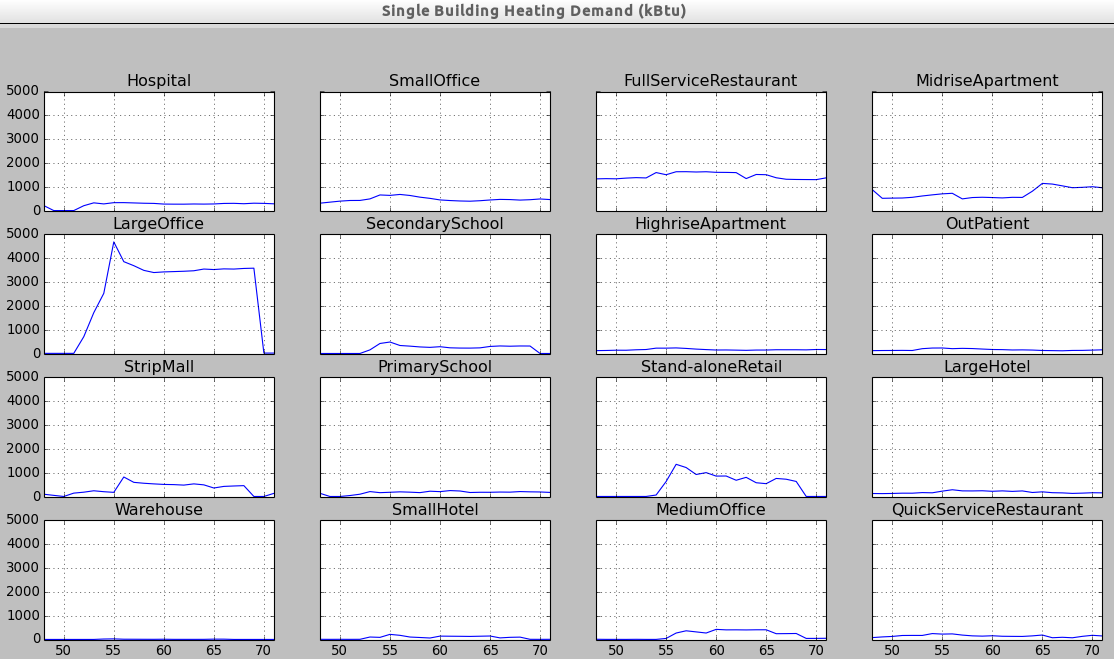
\includegraphics[width=0.7\linewidth]{dayDmdDiff.png}
    \caption{Space heating demand on 1/1/2015 of the 16 prototype
      buildings}
    \label{fig:dayDmdDiff}
  \end{figure}

\item The weekly demand pattern is different between different
  building types. In the example of \fref{fig:weekDmdDiff}, the Large
  Office, the Primary School, the Stand-alone Retail have strong
  weekday-weekend difference, while the rest of the building types
  have stable demand throughout the week.
  \begin{figure}[h!]
    \centering
    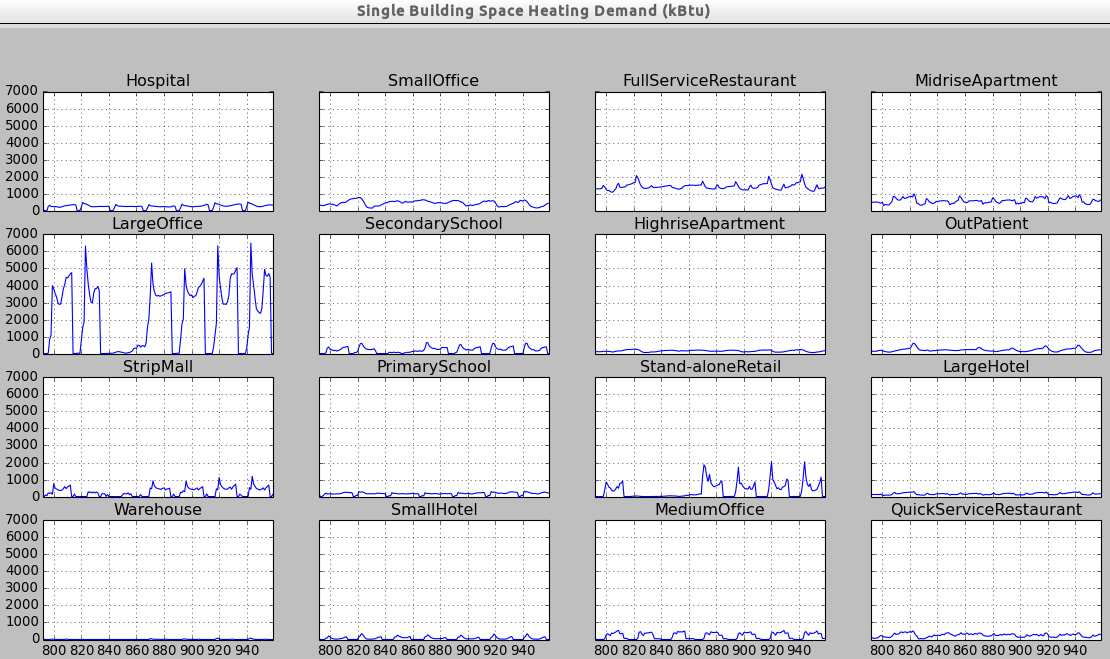
\includegraphics[width=0.7\linewidth]{weekDmdDiff.png}
    \caption{Space heating demand from 2/3/2015 to 2/10/2015 of the 16
      prototype buildings}
    \label{fig:weekDmdDiff}
  \end{figure}

\item In the use case study of identification of energy recovery
  opportunities, users could see the quantity of reject heat
  production and space heating demand of the group of buildings. They
  can observe the weekly pattern of the reject heat supply and the
  space heating demand are not co-incident: reject heat production in
  weekends is low while space heating demand in weekends is high
  (\sref{useCase1}).

\item In the use case study of CHP sizing, users can observe that the
  heating and electricity demand for the community have very different
  weekly demand behavior: electricity demand has strong
  weekday-weekend pattern with weekday having high demand and weekend
  having low demand, while heating demand does not have as strong a
  weekday-weekend pattern. (\sref{sec:CHPsize}).
\end{itemize}

\section{Limitations and Further Development}
The current project presented an initial implementation of a dynamic
energy map with the focus on spatial-temporal energy profile
visualization. Due to limited time and resources, there are many
improvement to be realized in the next stage development:

\begin{itemize}
\item Input data

  Urban level simulation software is not used in the energy profile
  generation. This leads to simplified assumptions of the influence of
  micro-climate in an urban environment on energy demand of buildings
  and the whole community. The building height and urban density could
  influence the exterior shading and could influence buildings'
  heating cooling and electricity demand: Ratti et al.\ analyzed the
  urban texture including surface-to-volume ratio (the total surface
  area over the total building volume), the ratio of passive zone
  (``quantify the potential of each part of a building to use
  daylight, sunlight and natural ventilation''~\cite{Ratti2005762}) to
  non-passive zone, and self-shading on the urban level energy demand
  with DEM models and LT simulation method in London, Toulouse and
  Berlin~\cite{Ratti2005762}. They discovered that the high ratio of
  passive zone has a strong positive effect on urban level energy
  demand reduction. Steemers discovered that in an $400 \times 400$
  region of London, doubling urban density results in a 25\% increase
  with the plot ratio ranging from 1.25:1 to
  5:1~\cite{Steemers20033}. The energy impact of urban environment
  configurations including urban density and the spatial distribution
  of building height could potentially be conveyed with the dynamic
  energy map with 3D map sequences. However as a result of the
  stand-alone assumption in commercial prototype building models, this
  layer of information is not demonstrated in the dynamic energy map
  in the current project.

  The current project focuses mainly on the energy demand information
  of heating cooling and electricity. The only energy supply parameter
  included is the cooling-induced reject heat. One of the major goal
  of energy mapping is to present detailed information of energy
  supply and energy demand and suggest possible connections that
  better matches the demand and supply. In order to fully realize the
  function of an energy map, adding high space-time resolution supply
  side information is crutial. In the further development of the
  project, supply side information, especially renewable energy supply
  assessment should be added to the dynamic energy map and the
  ``opportunity region'' where supply well meets the demand will also
  be calculated and depicted on the map. Different from the static
  map, the temporal changing of the size and location of the focus
  area will also be depicted on the next version of the dynamic energy
  map. The newly added layers of various energy supply and opportunity region
  could pose new challenges of map design and data visualization as a
  result of the potential overflow of information. Further investment
  of proper spatial-temporal data visualization method could also
  become another topic of the next stage development of the project.

  The matching of energy demand and supply include not only matching
  in energy quantity but also energy quality in terms of exergy
  ~\cite{Dobbelsteen2013}. The current map interface does not contain
  exergy information. Further development could add exergy information
  in order to facilitate the design of energy cascading and the design
  of a ``net-zero exergy district''~\cite{K20141077}.

\item Visualization

  In the data classification step, the break point is acquired with
  quantile classification method as is discussed in
  \sref{dataClassification}. Further analysis of building science
  context based break point selection, such as critical value for
  mechanical equipment sizing or minimum recoverable heat considering
  transmission loss etc., should be taken into consideration in the
  next stage development of the project.
  
\item Data Sharing
  
  As is envisioned in the study of Baird et al.\ , an on-line platform
  is needed to facilitate data access, model sharing and advanced
  analysis of a dynamic energy map~\cite{baird2014}. The current
  implementation of the dynamic energy map is a stand-alone
  tool. Bringing the current stand-alone map to an online platform
  could be one of the topics of the next stage development.

\item Technical issue

  As a result of the dependence on an existing modeling software,
  CityEngine, for image generation, user could not create community
  design and compare design alternatives on the current interface;
  user control over data classification and legend selection are not
  realized either. To solve this problem, a 3D model importing and
  rendering function should be added to the current map to facilitate
  the performance-based geo-design method in the community energy
  planning.

\item Analytical ability

  The primary focus of the project at the current stage is on energy
  demand data visualization, thus the decision support routines
  including district system specification, the financial assessment
  and additional land use constraints are not added to the current
  interface. Equipping the current dynamic energy map with the
  analysis abilities above could be one of the topics of the next
  stage development.
  
  In the use case of identification of the energy recovery
  opportunity, the calculation of energy recovery potential has a
  simplified assumption that all reject heat could be recovered.  In
  the further development of the project, the research would add more
  detailed analysis of reject heat taken detailed system configuration
  into account.
  
  Another analytical ability is to calculate the ``opportunity
  region'' where there is a high potential of the better matching of
  the supply and the demand. Since the demand and supply changes over
  time, the ``opportunity region'' will also change over both space
  and time. For a dynamic energy map, the change of the location and
  service area of the ``opportunity region'' could also be
  depicted. This information could help planners create time-of-use
  strategies that adapts to the spatial-temporal changing of region
  with better matching of supply and demand.
  
  Another crucial feature to be developed in the next stage is the
  generic analytical functions of space-time data. Although
  visualization of space-time energy profile on the community map
  facilitates the recognition of the general pattern of energy demand
  and supply, more accurate description and validation of the pattern
  discovered from the process of visualization needs to be tested
  against more rigorous mathematical analysis of space-time data. For
  example, the buildings with large demand variations can pose
  challenges to the district system design because they'll require the
  capacity of the district system to be large enough to meet their
  peak demand, causing the district local plant to run on its
  non-optimal output for a longer period. If these types of buildings
  are paired with buildings with complimentary energy demand
  (\fref{fig:plotAll}), the total demand variation of the group of
  buildings would be reduced. However to define what is
  ``complimentary'' demand is not easy, especially when all buildings
  have different energy demand profile. A brute force approach that
  tries out all possible combinations of building demand profiles and
  check if they reduce the aggregated demand is not feasible because
  the time spent to solve the problem grow exponentially with the
  number of distinct building profiles. For the current dynamic map
  model, with 68 buildings and 9 different building energy demand
  profiles involved, the total number of trials could be about
  $2^9 = 512$. For the current community model, if all buildings have
  their own demand profile, the total number of trials will be
  $2^{68}$, about $3\times10^{20}$. Obviously this method will not
  feasible for large communities. In this case, k-mean clustering
  method ~\cite{kmean2015} can be used to classify the building energy
  demand profiles into groups with similar demand behavior and reduce
  the distinct building profile type to a manageable amount. Adding
  such advanced data analysis functions could provide more informative
  land use design suggestions to improve the overall community energy
  performance.

\end{itemize}